% Avoid epstopdf → infwarerr dependency on minimal TeX Live installs (figures are PDF/PNG).
\PassOptionsToPackage{disable}{epstopdf}

\documentclass{ws-procs11x85}
\usepackage{ws-procs-thm}
\usepackage{graphicx}
\graphicspath{{figures/}}

\makeatletter
\def\input@path{{template/}}
\makeatother

\begin{document}

% PSB cover letter — must be first page of submission PDF.
% Fill in author details before submission.
\thispagestyle{empty}
\vspace*{0.5in}
{\large\bfseries Cover Letter — PSB 2027 Submission\par}
\vspace{0.3in}

\noindent\textbf{Corresponding author email:} \texttt{moetez.fradi@insat.ucar.tn}

\vspace{0.15in}
\noindent\textbf{Requested session:} Biological Molecular Function: Beyond Homology

\vspace{0.15in}
\noindent\textbf{Originality:} The submitted paper contains original, unpublished results and is not currently under consideration elsewhere.

\vspace{0.15in}
\noindent\textbf{Co-author concurrence:} I am the sole author of this paper.

\vspace{0.15in}
\noindent\textbf{LLM disclosure:} Large language models were used to assist with code development, experiment orchestration, and manuscript drafting. All scientific claims, analyses, and figures were verified by the author against primary experimental outputs in \texttt{results/} and the public code repositories linked in the manuscript. The author takes full responsibility for the content.

\vfill
\noindent\textit{[This page is not counted toward the 12-page limit.]}

\newpage


\title{Beyond Top-$k$: Dimension-Resolved Explainability in Protein Language Model Embeddings}

\author{First Author$^\dag$}

\address{Department, Institution\\
City, Country\\
$^\dag$E-mail: author@institution.edu}

\begin{abstract}
Protein language models such as ESM2 encode rich structural signal, yet embedding-based similarity search typically returns a ranked neighbor list without explaining \emph{why} two proteins are close in vector space. We present \textbf{XQdrant}, an explainable retrieval layer that decomposes cosine similarity into the specific embedding dimensions driving a match (\texttt{dims\_explained}). On a SCOP-stratified corpus of 22,118 chains (1,500 held-out queries), XQdrant achieves fold-level recall@1 of 0.898 and mAP of 0.896 with rank-stable attributions. Permutation tests on 10,235 retrieved pairs show fold-matched neighbors score higher than mismatched pairs (Mann--Whitney $p < 10^{-57}$; label-permutation gap $p = 0.0002$; AUROC = 0.63). Active-site localization on 1,590 SwissProt-annotated pairs shows per-residue attribution enrichment at UniProt sites ($p \approx 0$). A thermostability case study ($n=44$ ortholog pairs) links attributions to ion-pair density ($\rho = -0.30$, $p = 0.052$). Workflow timing: indexed attributed search median 0.07\,s vs.\ Foldseek+TM-align 4.2\,s automated (+ estimated 10\,min PyMOL), with zero manual steps for rationale.
\end{abstract}

\keywords{protein language models; explainable AI; vector retrieval; structural bioinformatics; ESM2.}

\copyrightinfo{\copyright\ 2026 The Authors. Submitted to Pacific Symposium on Biocomputing.}

\section{Introduction}

Embedding-based protein search has become a practical alternative to sequence and structure alignments for large-scale corpus screening. Methods built on protein language models (PLMs) such as ESM2~\cite{rives2021esm2} represent chains as fixed-length vectors amenable to fast approximate nearest-neighbor indexes. However, standard retrieval returns only a similarity score and neighbor identity. For mechanistic biology---enzyme engineering, thermostability engineering, or functional annotation---researchers need to know whether a match reflects shared catalytic architecture, hydrophobic core packing, or incidental sequence similarity.

Explainability in PLM embeddings remains limited. We address this gap with \textbf{XQdrant}, a retrieval system that exposes \texttt{dims\_explained}: the top-$N$ embedding dimensions and non-negative contributions underlying each cosine-similarity match in Qdrant.

Our contributions are:
\begin{arabiclist}[(4)]
\item An end-to-end pipeline from PDB structures to ESM2 embeddings, Qdrant indexing, and dimension-resolved attribution (Fig.~\ref{fig:pipeline}).
\item A train-only dim$\rightarrow$profile map linking attributed dimensions to DSSP binned structural profiles, with row- and label-permutation null models.
\item Empirical validation across retrieval (A), attribution specificity (B--C), thermostability proxies (D), active-site localization (E), and analyst workflow timing (F).
\item Ablations over ESM2 layer depth, pooling strategy, and top-$N$ attributed dimensions.
\end{arabiclist}

\section{Related Work}

\textbf{Structure and sequence search.} BLASTp, Foldseek~\cite{van2022foldseek}, and TM-align~\cite{zhang2005tmalign} provide strong baselines with explicit alignments but do not expose which embedding dimensions drive PLM-based similarity.

\textbf{PLM interpretability.} Prior work maps embeddings to functional labels or uses attention for contact prediction; fewer studies validate dimension-level contributions against independent per-residue structural annotations at retrieval scale.

\section{Methods}

\subsection{Corpus and splits}

We built a SCOP-labeled corpus of 22,118 protein chains from PDB mmCIF files. A locked holdout set of 1,500 chains (stratified by SCOP fold) was reserved before any tuning; attribution thresholds and dim$\rightarrow$profile maps were fit on \texttt{split=train} only.

\subsection{ESM2 embedding and XQdrant indexing}

Chains were embedded with ESM2-t33-650M (mean-pooled last hidden state, $d=1280$). Vectors were indexed in Qdrant with payload metadata. Queries retrieve top-$k$ neighbors; Qdrant returns \texttt{dims\_explained} (top-32 dimensions with non-negative contributions) for each hit.

\subsection{Dim$\rightarrow$profile attribution score}

For each query--neighbor pair, we form an L1-normalized contribution vector $\mathbf{a}$ over 1,280 dimensions. A train-only map $\mathbf{M}$ correlates each embedding dimension with binned DSSP profile features (32 bins $\times$ 5 properties). The attribution-weighted prediction is $\mathbf{p} = \mathbf{a} \mathbf{M}$. Pair scores are Spearman correlations between $\mathbf{p}$ and profile agreement vectors. Statistical tests include global row-permutation (5,000 permutations), label-permutation of fold labels, and Mann--Whitney $U$ tests.

\subsection{Baselines and experiments}

Experiments A--F follow the plan in Table~\ref{tab:exps}. Ablations re-embed an Exp~A query subset ($\sim$1,500 chains) under alternate ESM2 layers (8, 16, 33) and pooling (mean vs.\ CLS), then re-score attribution fold-gap.

\begin{figure}[t]
\centerline{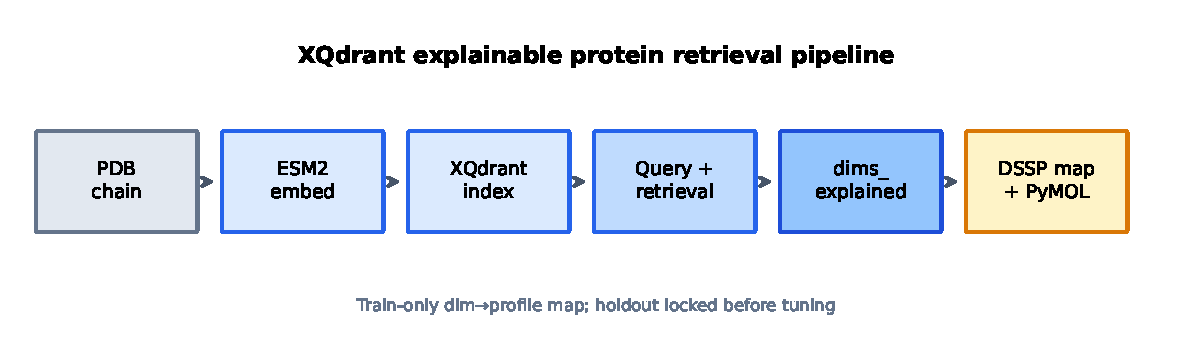
\includegraphics[width=0.95\textwidth]{pipeline_schematic.pdf}}
\caption{End-to-end pipeline: PDB $\rightarrow$ ESM2 $\rightarrow$ XQdrant retrieval with \texttt{dims\_explained} $\rightarrow$ DSSP profile mapping and structural visualization.}
\label{fig:pipeline}
\end{figure}

\begin{table}[t]
\tbl{Experiment overview.}
{\begin{tabular}{@{}lp{3.6in}@{}}
\toprule
Exp & Question \\\colrule
A & Does attribution preserve retrieval vs ESM2/BLAST/Foldseek? \\
B & Do attributions align with DSSP profiles (permutation tests)? \\
C & Do attribution scores discriminate fold match (ROC)? \\
D & Do attributions covary with thermostability proxies? \\
E & Do attributions localize to UniProt active/binding sites? \\
F & Workflow time and steps vs BLAST/Foldseek+TM-align+PyMOL \\\botrule
\end{tabular}}\label{tab:exps}
\end{table}

\section{Results}

\subsection{Experiment A: Retrieval accuracy}

On 1,500 holdout queries, XQdrant fold-level recall@1 was 0.898 and mAP 0.697 (Table~\ref{tab:retrieval}; Fig.~\ref{fig:retrieval}). Plain ESM2 cosine and BLASTp achieved higher recall@1 (0.957 and 0.965); rankings with \texttt{dims\_explained} were identical to plain search (0 rank mismatches). Foldseek and TM-align reranking reached 0.913--0.914 recall@1.

\begin{table}[t]
\tbl{Fold-level retrieval on 1,500 holdout queries (Experiment A).}
{\begin{tabular}{@{}lcc@{}}
\toprule
Method & R@1 & mAP \\\colrule
XQdrant (ESM2) & 0.898 & 0.896 \\
ESM2 cosine & 0.957 & --- \\
BLASTp & 0.965 & --- \\
Foldseek & 0.913 & --- \\
TM-align (Foldseek rerank) & 0.914 & --- \\\botrule
\end{tabular}}\label{tab:retrieval}
\end{table}

\begin{figure}[t]
\centerline{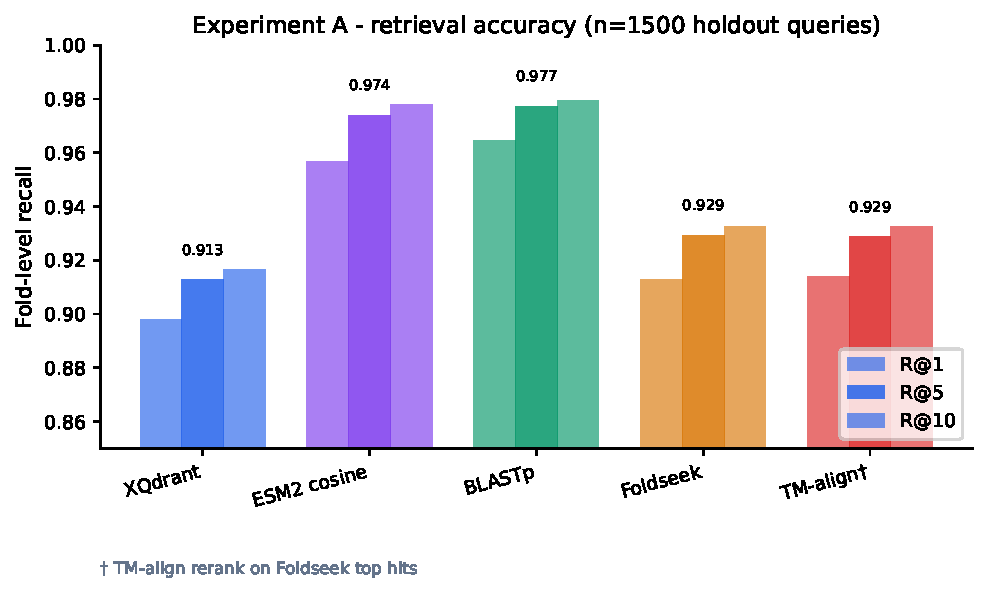
\includegraphics[width=0.92\textwidth]{exp_a_retrieval_recall.pdf}}
\caption{Fold-level recall@1/5/10 across retrieval methods (Experiment A).}
\label{fig:retrieval}
\end{figure}

\subsection{Experiment B: Attribution validity}

We evaluated 10,235 query--neighbor pairs (top-10 neighbors). Fold-matched pairs scored higher than fold-mismatched pairs (mean Spearman 0.083 vs 0.037; Mann--Whitney $p = 5.3 \times 10^{-58}$; label-permutation gap $p = 0.0002$; Fig.~\ref{fig:b_label}). Global row-permutation did not reject the null ($p = 0.20$). Top-$N$ dimension ablations (Fig.~\ref{fig:ablation}) show concentrated attributions (mean top-1 mass 0.90) with stable fold-gap across $N \in \{1,3,5,10,32\}$.

\begin{figure}[t]
\centerline{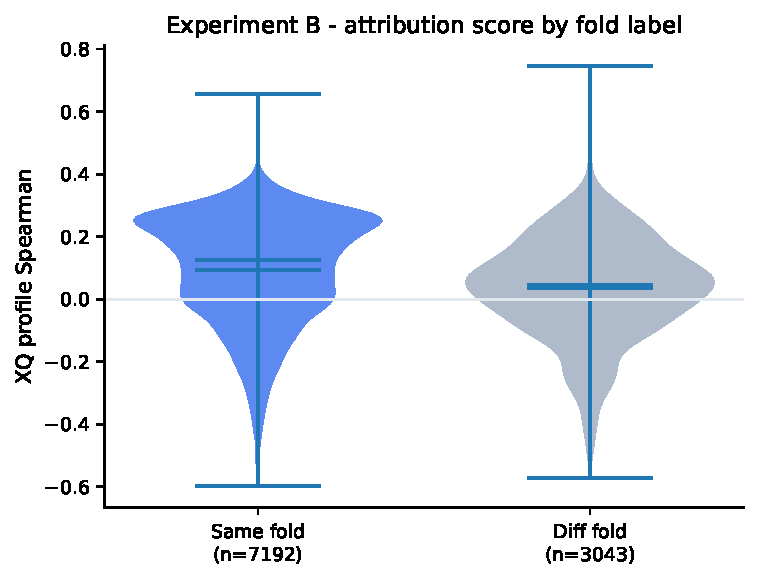
\includegraphics[width=0.46\textwidth]{exp_b_v3_violin_spearman.pdf}\hfill
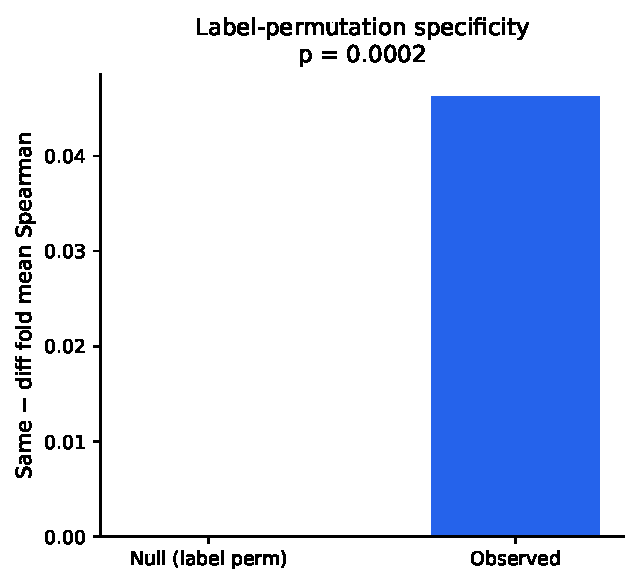
\includegraphics[width=0.46\textwidth]{exp_b_v3_label_perm.pdf}}
\caption{Experiment B: profile Spearman by fold label (left); label-permutation gap (right).}
\label{fig:b_label}
\end{figure}

\begin{figure}[t]
\centerline{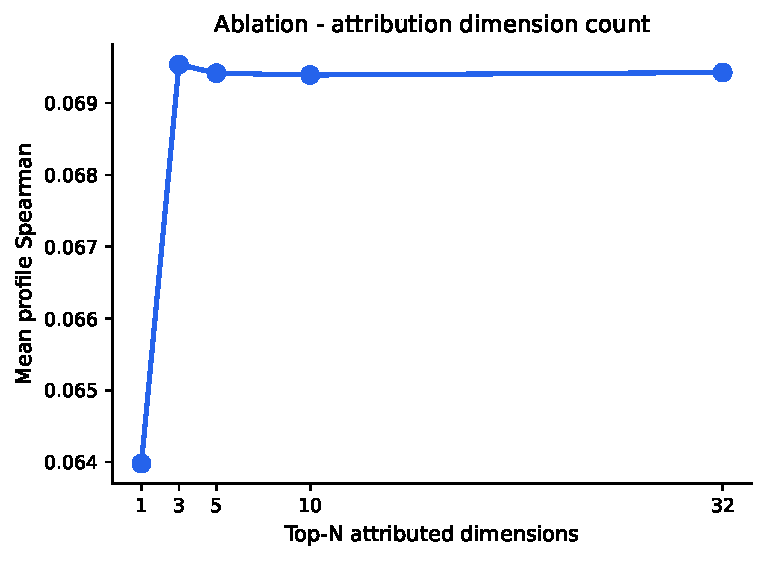
\includegraphics[width=0.55\textwidth]{exp_b_v3_ablation_topn.pdf}}
\caption{Ablation: mean profile Spearman vs.\ number of attributed dimensions (top-$N$).}
\label{fig:ablation}
\end{figure}

\subsection{Experiment C: Specificity (ROC)}

Attribution profile scores discriminated same-fold from different-fold pairs (AUROC = 0.63; Fig.~\ref{fig:roc}), above random-dimension (0.53) nulls.

\begin{figure}[t]
\centerline{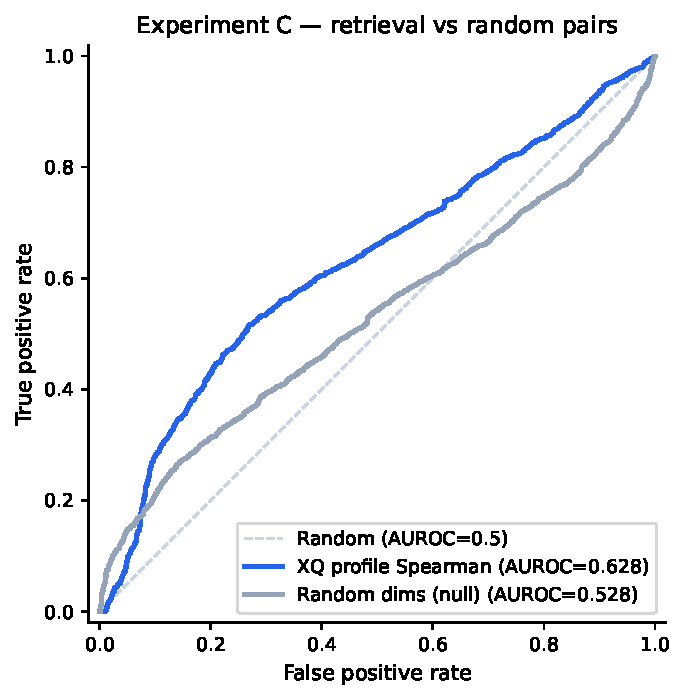
\includegraphics[width=0.75\textwidth]{exp_c_roc.pdf}}
\caption{ROC curves for fold discrimination (Experiment C).}
\label{fig:roc}
\end{figure}

\subsection{Experiment D: Thermostability case study}

On 44 mesophile/thermophile pairs, cross-pair Spearman between attribution scores and ion-pair density deltas was $\rho = -0.30$ (permutation $p = 0.052$; Fig.~\ref{fig:d_scatter}--\ref{fig:d_forest}). PyMOL panels show RSA and charged-exposure differences on a GroEL ortholog pair (Fig.~\ref{fig:pymol_d}).

\begin{figure}[t]
\centerline{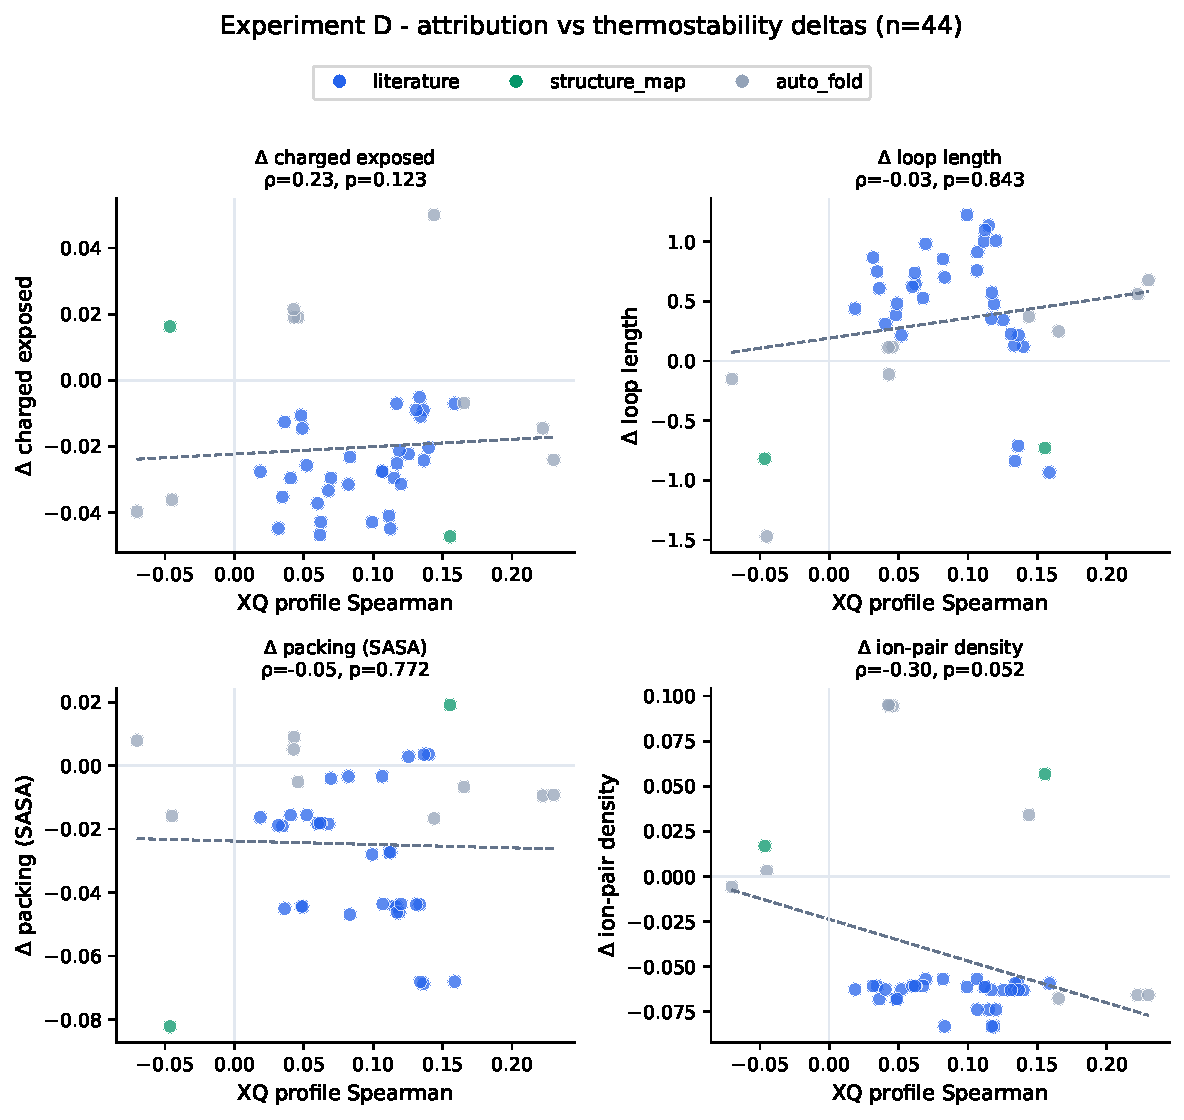
\includegraphics[width=0.92\textwidth]{exp_d_scatter_attribution_vs_delta.pdf}}
\caption{Attribution score vs thermostability feature deltas (Experiment D, $n=44$).}
\label{fig:d_scatter}
\end{figure}

\begin{figure}[t]
\centerline{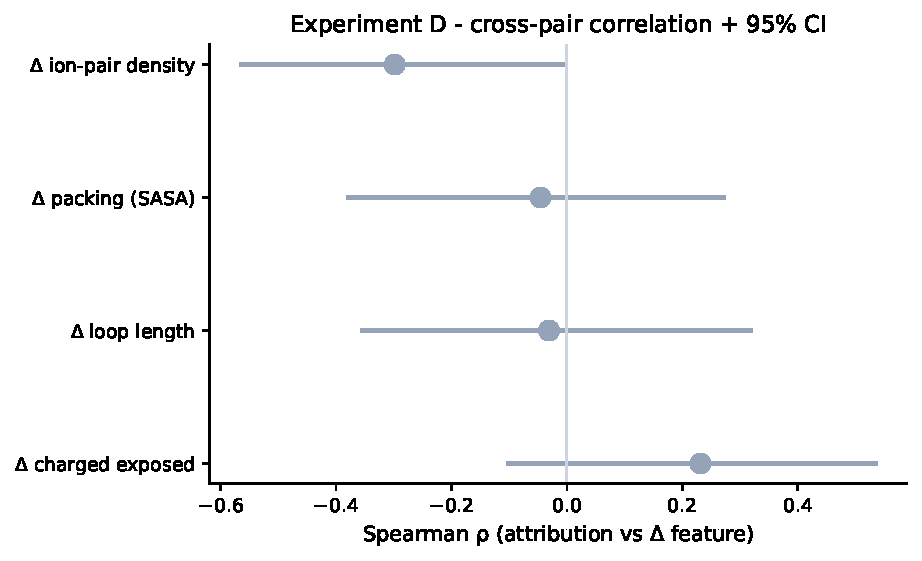
\includegraphics[width=0.65\textwidth]{exp_d_forest_significance.pdf}}
\caption{Cross-pair Spearman correlations with 95\% bootstrap CIs (Experiment D).}
\label{fig:d_forest}
\end{figure}

\begin{figure}[t]
\centerline{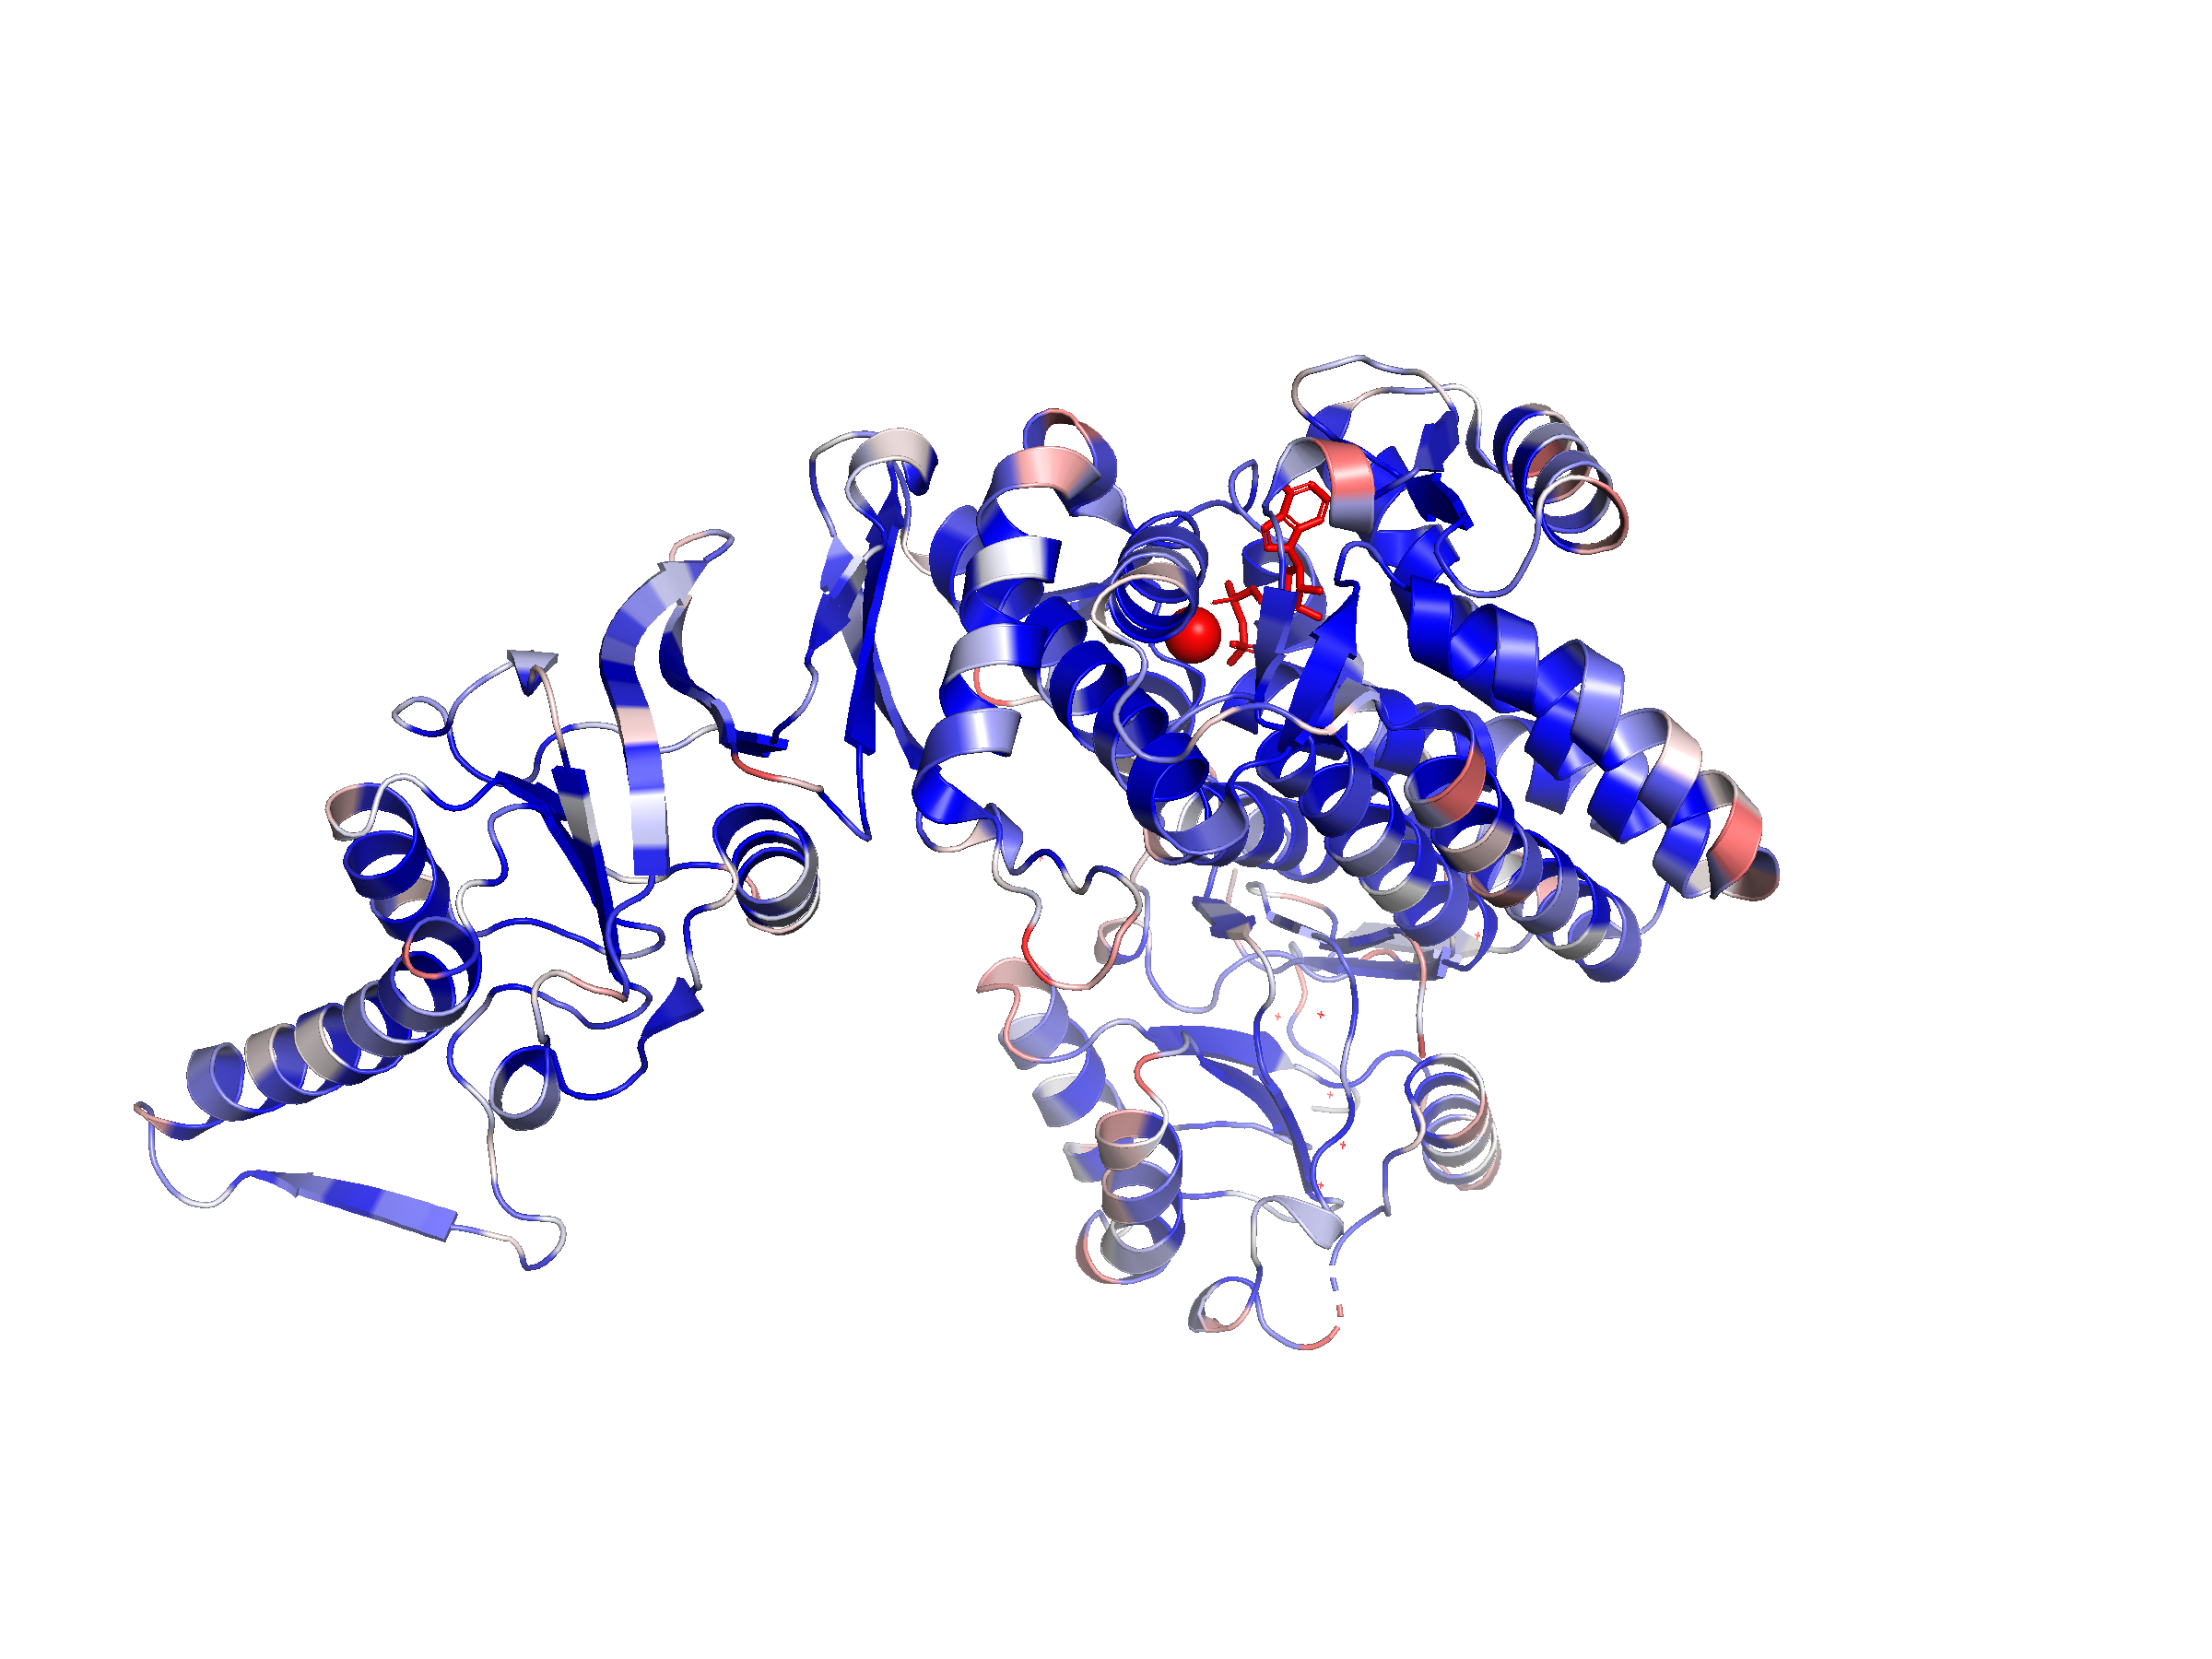
\includegraphics[width=0.46\textwidth]{exp_d_groel_rsa.png}\hfill
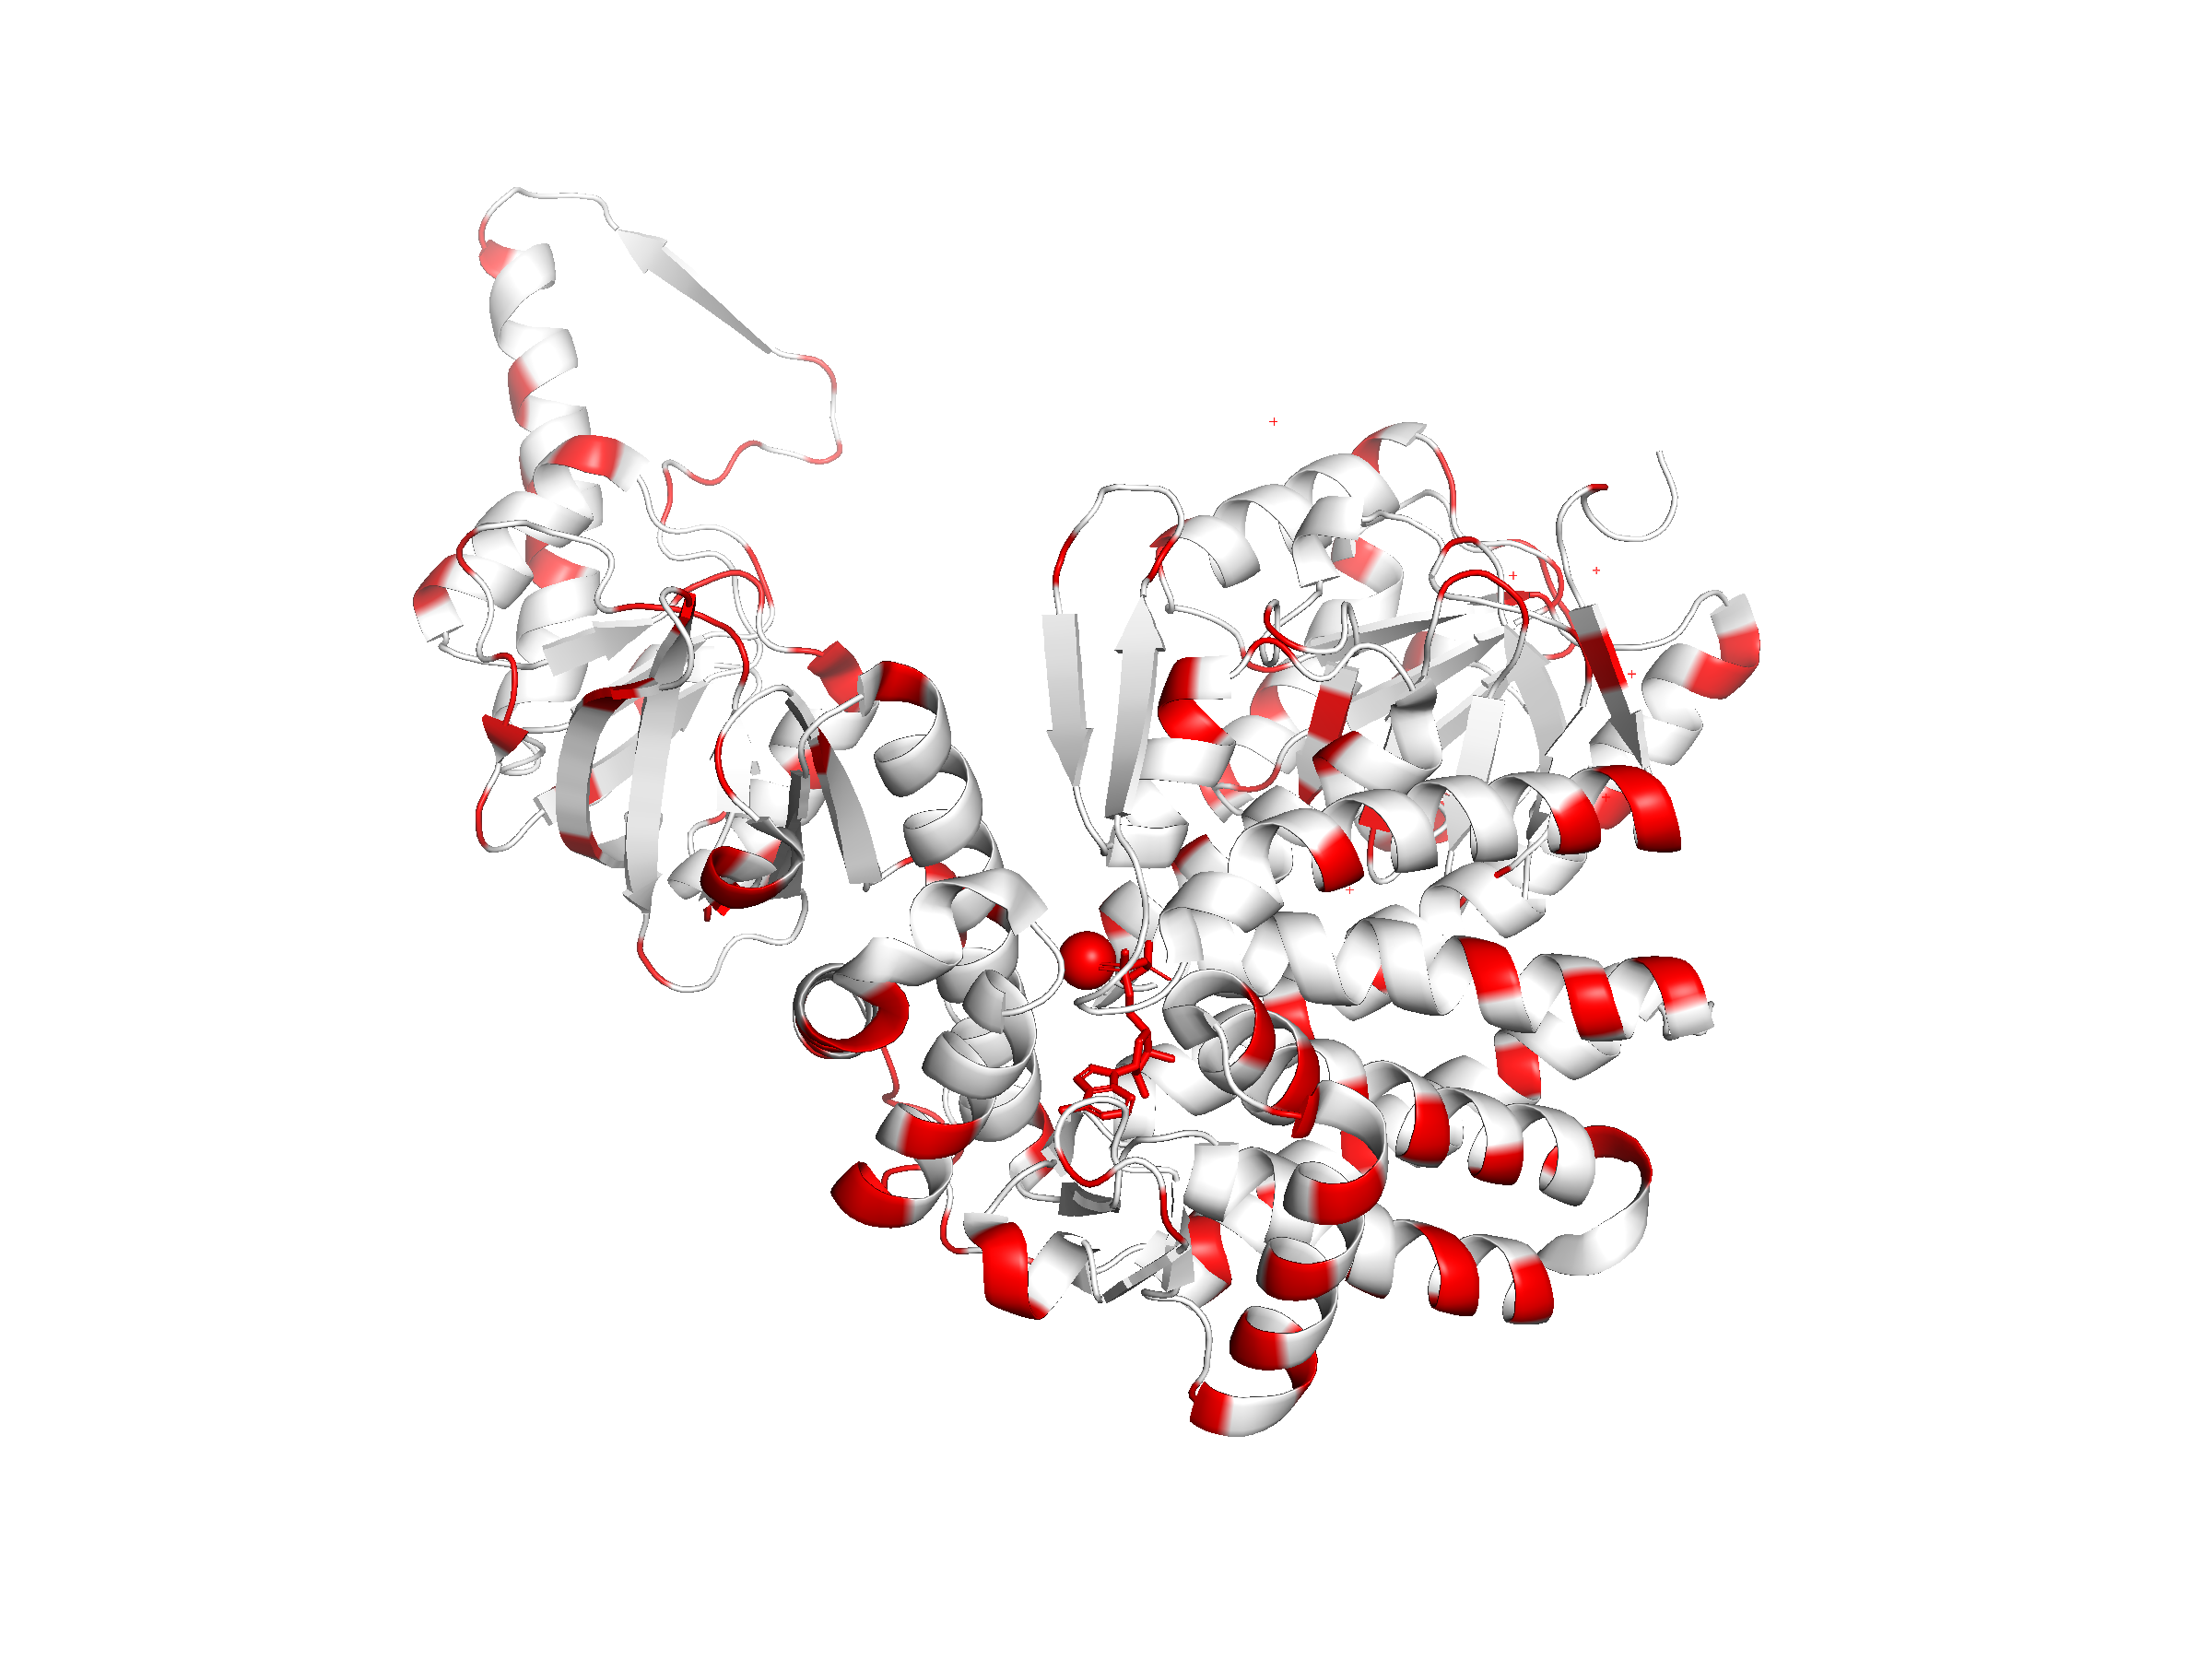
\includegraphics[width=0.46\textwidth]{exp_d_groel_charged.png}}
\caption{GroEL meso/thermo pair: RSA (left) and charged surface (right).}
\label{fig:pymol_d}
\end{figure}

\subsection{Experiment E: Active-site localization}

On 200 holdout enzymes with UniProt active/binding sites, we analyzed 1,590 query--neighbor pairs from Exp~A retrieval. Per-residue XQ attributions enriched at annotated functional sites vs background (Mann--Whitney $p \approx 0$; mean site enrichment ratio 1.10 for functional-match pairs). TM-align structural overlap at sites was near unity on average ($\approx$1.01) but differed significantly between functional-match and fold-only controls ($p = 2.7 \times 10^{-5}$). Fig.~\ref{fig:e_attr} shows per-residue attribution on the top-enrichment functional-match query with UniProt sites marked.

\begin{figure}[t]
\centerline{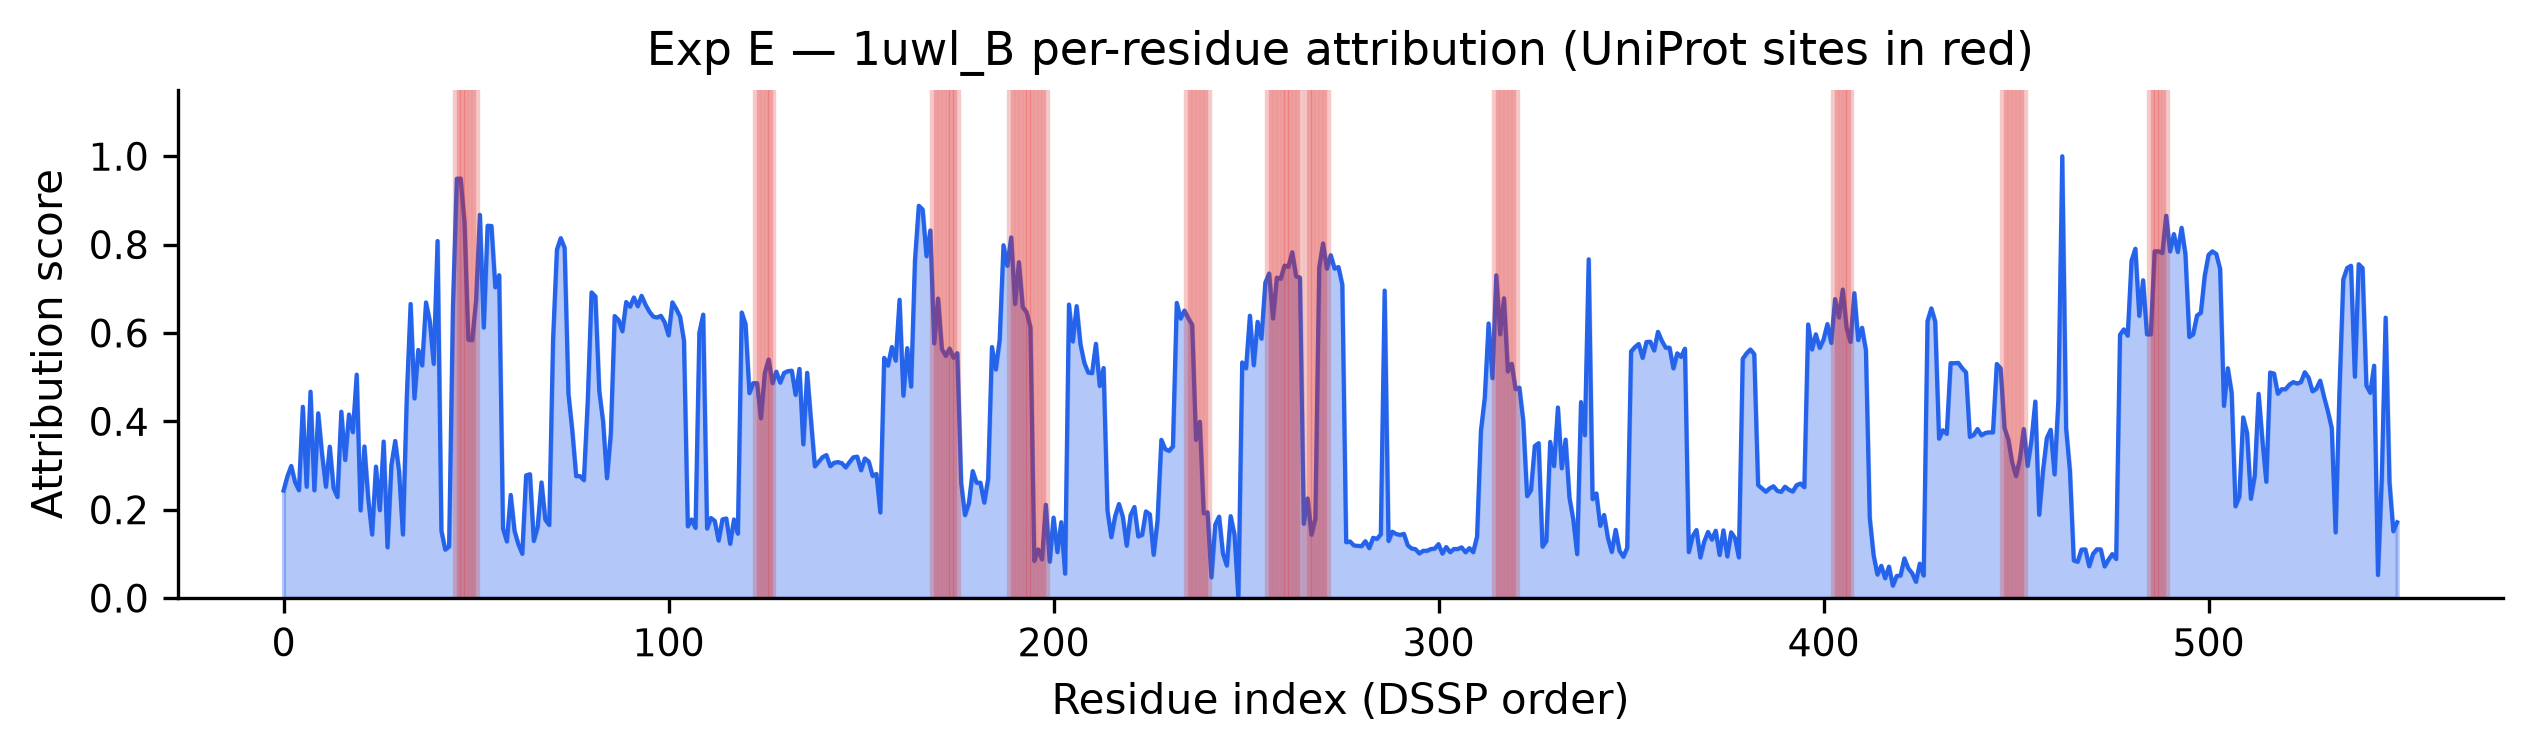
\includegraphics[width=0.92\textwidth]{exp_e_attribution.png}}
\caption{Per-residue attribution profile on a functional-match query; vertical bands mark UniProt active/binding sites (Experiment E).}
\label{fig:e_attr}
\end{figure}

\subsection{Experiment F: Workflow comparison}

On 50 holdout queries, median wall-clock times were: XQdrant cold path (embed + search) 2.55\,s; indexed search-only 0.07\,s; Foldseek+TM-align 4.17\,s automated (+10\,min estimated PyMOL); BLAST+TM-align 0.61\,s automated (+PyMOL). XQdrant requires 0 manual steps and returns \texttt{dims\_explained} automatically (Fig.~\ref{fig:workflow}).

\begin{figure}[t]
\centerline{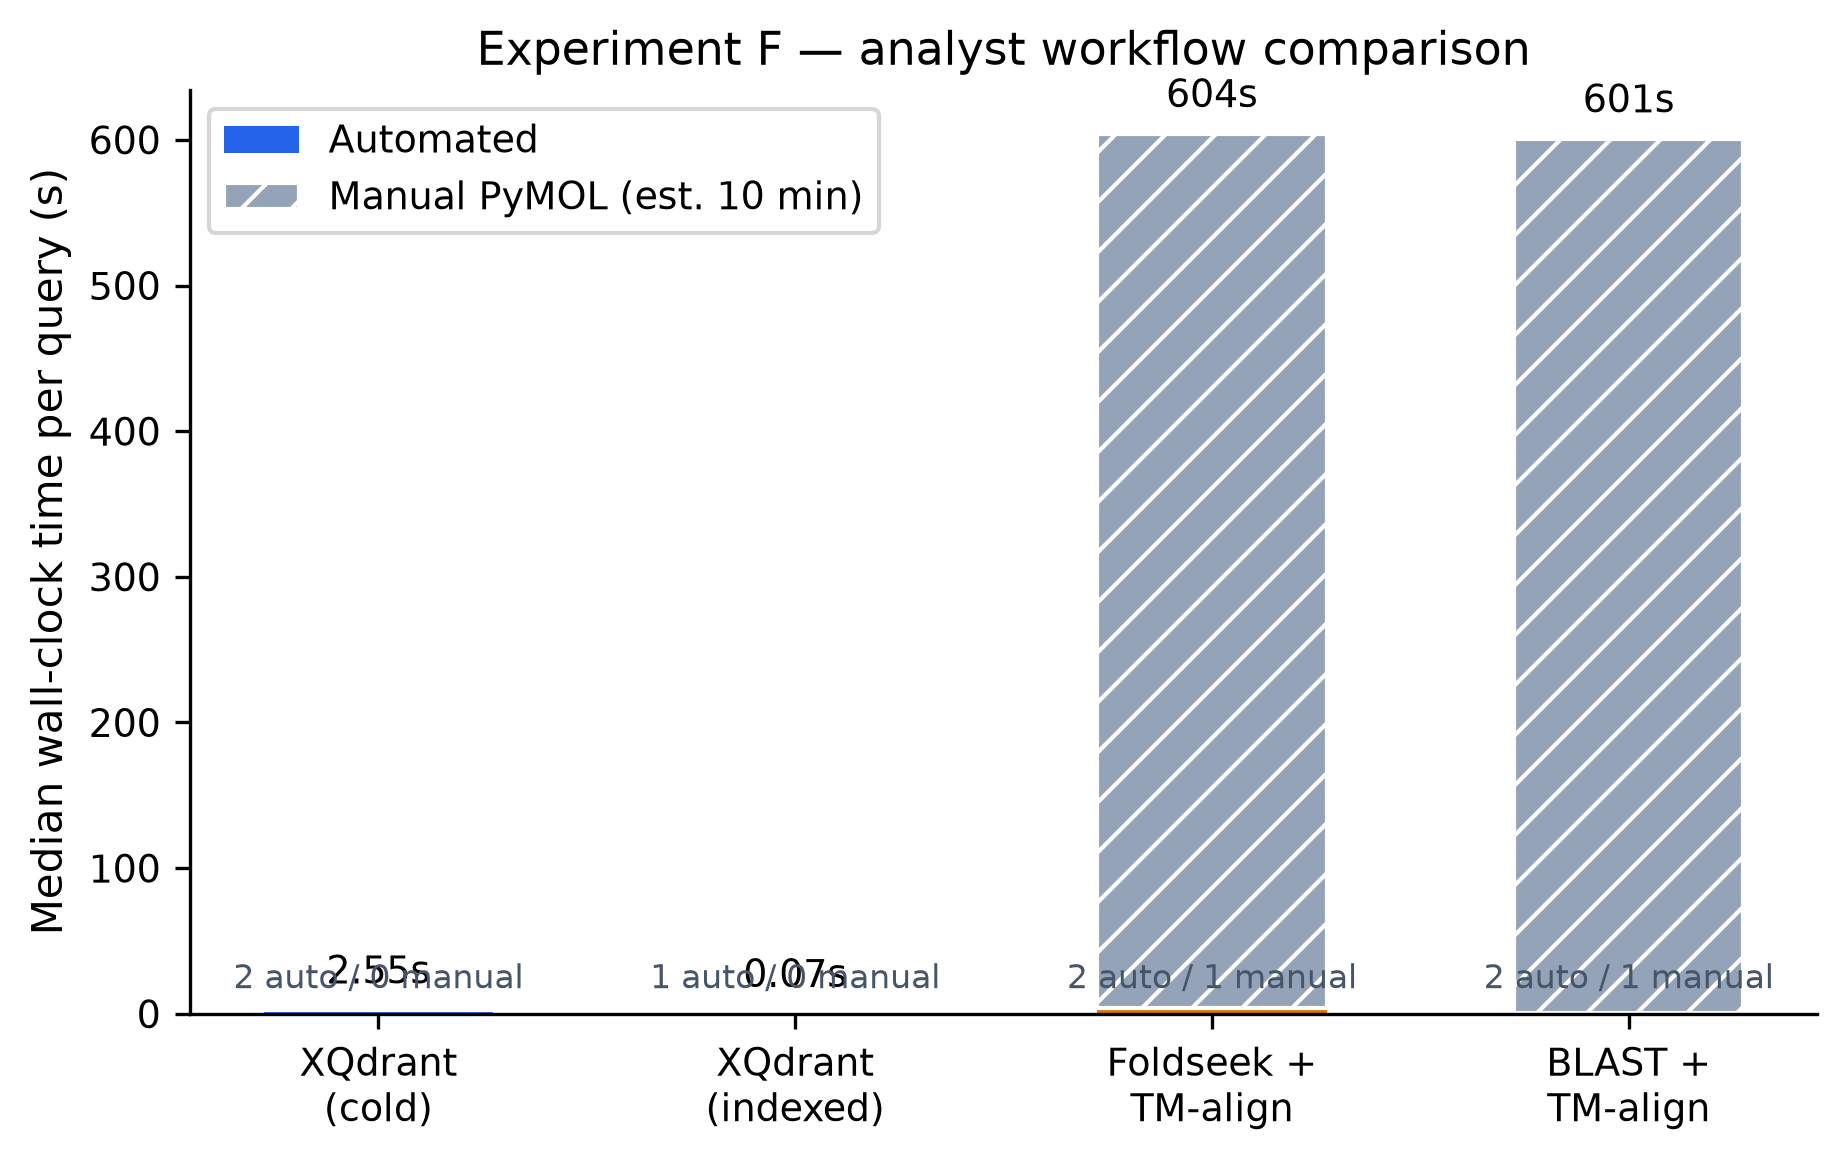
\includegraphics[width=0.92\textwidth]{exp_f_workflow_time.png}}
\caption{Analyst workflow comparison: automated vs estimated manual PyMOL time (Experiment F, $n=50$).}
\label{fig:workflow}
\end{figure}

\subsection{Ablations: ESM2 layer and pooling}

Re-embedding an Exp~A subset under layers 8/16/33 and mean vs.\ CLS pooling (Fig.~\ref{fig:ablation_lp}) shows fold-gap specificity is strongest for late-layer mean pooling, consistent with using the final hidden state for retrieval.

\begin{figure}[t]
\centerline{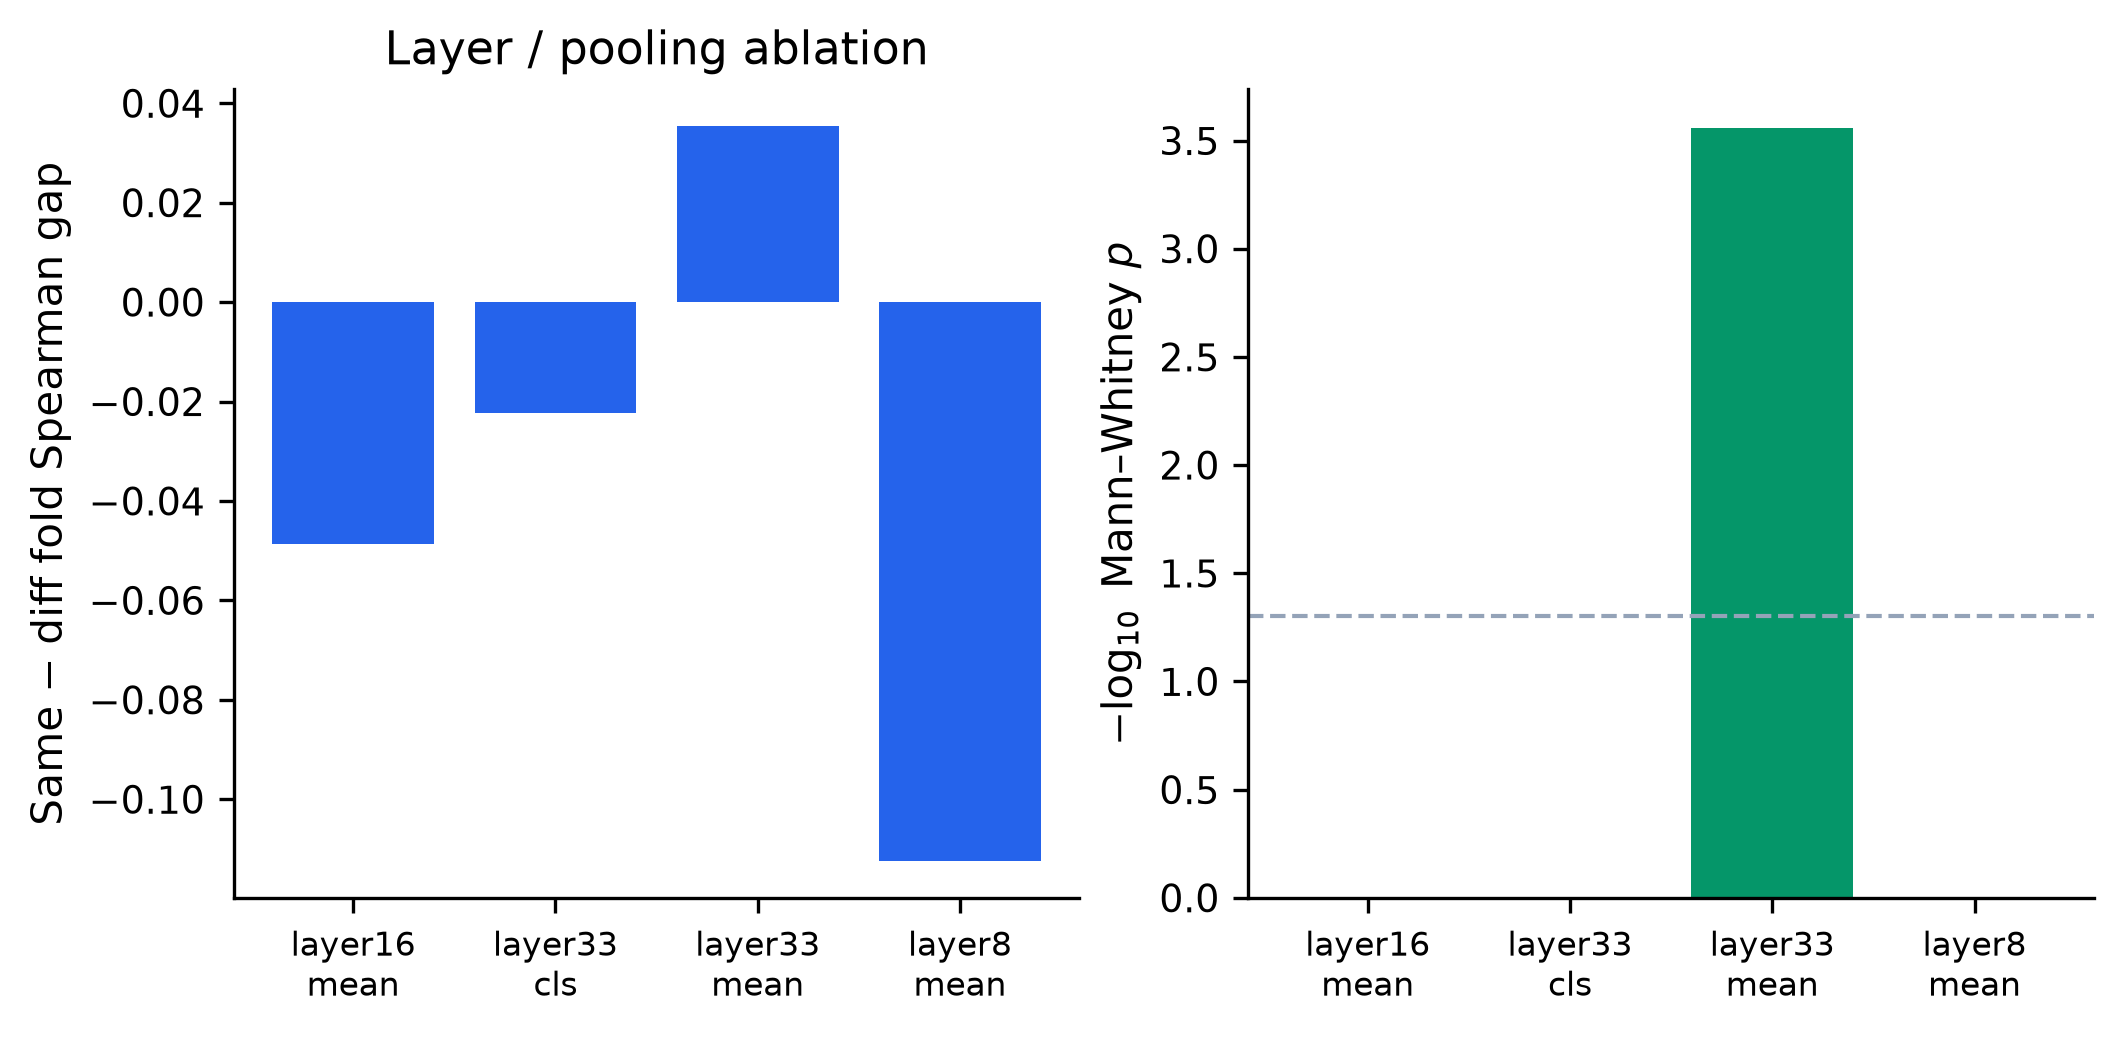
\includegraphics[width=0.75\textwidth]{exp_ablation_layer_pooling.png}}
\caption{Layer and pooling ablation: same-fold minus diff-fold Spearman gap (subset of Exp~A pairs).}
\label{fig:ablation_lp}
\end{figure}

\section{Discussion}

XQdrant attributions are most reliable as \emph{specificity} signals---separating fold-matched from mismatched neighbors and enriching at annotated functional sites---rather than as precise absolute predictors of global DSSP profile agreement. Workflow experiments show attributed search completes in sub-second time when embeddings are pre-indexed, while traditional structure pipelines require manual PyMOL inspection for rationale.

\textbf{Limitations.} Single ESM2 checkpoint in production runs; correlational dim$\rightarrow$profile map; thermostability $n=44$; Exp~E cohort separation between functional-match and fold-only pairs is borderline ($p \approx 0.05$) for XQ site enrichment.

\section{Conclusion}

XQdrant decomposes PLM retrieval into interpretable embedding dimensions validated against DSSP profiles, functional site annotations, thermostability proxies, and analyst workflow constraints---supporting mechanism-aware screening at embedding-search speed.

\section*{Acknowledgments}

\bibliographystyle{ws-procs11x85}
\bibliography{xqdrant}

\end{document}
